
\documentclass{jtetiproposalskripsi}

%-----------------------------------------------------------------
%Disini awal masukan untuk data proposal skripsi
%-----------------------------------------------------------------
\titleind{SISTEM INFORMASI PENYEWAAN AULA
BERBASIS WEB PADA KANTOR PGRI KABUPATEN JEMBER}
\fullname{MOh Nasir}

\idnum{1200631015}

\approvaldate{10 Januari 2015}

\degree{Sarjana Komputer}

\yearsubmit{2015}

\program{Manajemen Informatika}

\headprogram{Triawan Adi cahyanto,M. Kom}

\dept{Manajemen Informatika dan Teknik Informatika}

\firstsupervisor{Triawan Adi cahyanto,M. Kom}
\firstnip{1976 0501 2002 12 1 002}

\secondsupervisor{Yeni dwi rahayu,M. kom}
\secondnip{1977 0131 2002 12 1 003}


%-----------------------------------------------------------------
%Disini akhir masukan untuk data proposal skripsi
%-----------------------------------------------------------------

\begin{document}

\cover

\approvalpage

%-----------------------------------------------------------------
%Disini akhir masukan untuk muka skripsi
%-----------------------------------------------------------------

%-----------------------------------------------------------------
%Disini awal masukan Intisari
%-----------------------------------------------------------------
\begin{abstractind}
Tujuan penelitian ini adalah untuk mempermudah kerja karyawan PT.
Kartika Buana Ayu yang mengelola gedung pertemuan Balai Kartini dalam
menyajikan suatu informasi dan mengolah data mengenai penyewaan gedung.
Dimana sebelumnya, proses penyampaian sistem informasi penyewaan gedung
yang digunakan belum terkomputerisasi dan dapat menyita banyak waktu. Se-
hingga tingkat kesalahan dalam mencari informasi serta mendata status penye-
waan gedung masih tinggi. Hal ini dapat membuat sistem penyewaan gedung
menjadi tidak terstruktur dan tidak terkendali dengan baik. Metode peneli-
tian yang digunakan meliputi metode kepustakaan, metode perancangan, dan
metode analisa yang mencakup survei serta pengamatan. Dari hasil peneli-
tian tersebut, dapat diambil kesimpulan bahwa karyawan PT. Kartika Buana
Ayu membutuhkan suatu sistem baru yang mempermudah kinerja karyawan,
menghemat waktu, serta mudah dijalankan, sehingga hasil pekerjaan karyawan
lebih terorganisir dan berjalan dengan baik. Dengan adanya sistem yang baru
ini juga diharapkan dapat memperkecil kesalahan yang dilakukan oleh karyawan
(human error), menghindari manipulasi data yang dilakukan oleh pihak yang
tidak bertanggung jawab, serta menjadi keunggulan tersendiri bagi perusahaan
yang mengedepankan kemajuan teknologi dengan menggunakan sistem yang
telah berbasis komputerisasi dan tersaji dalam satu sistem.


\bigskip
\textbf{Kata kunci} : \emph{SISTEM INFORMASI PENYEWAAN AULA, MySQL, PHP}.
\end{abstractind}
%-----------------------------------------------------------------
%Disini akhir masukan Intisari
%-----------------------------------------------------------------

\tableofcontents
\addcontentsline{toc}{chapter}{DAFTAR ISI}
\selectlanguage{bahasa}\clearpage\pagenumbering{arabic}\setcounter{page}{1}

%-----------------------------------------------------------------
%Disini awal masukan untuk Bab
%-----------------------------------------------------------------
\chapter{LATAR BELAKANG}

\section{Latar Belakang Masalah}
Pendataan administrasi pada manajemen Kantor PGRI Kabupaten Jember memerlukan ketepatan mekanisme dan penataan data yang teroganisir dan terjaga keamanannya dengan baik, seiring pesatnya kemajuan teknologi dan kemudahan yang ditawarkan didalamnya, kini instansi - instansi baik swasta maupun negeri mamanfaatkan fasilitas teknologi dalam pengolahan data-data yang dulu diolah secara manual diubah ke dalam pola komputerisasi yang dapat mempermudah proses penginputan dan pencarian data-data yang telah tersimpan dalam database. Database tersebut dibuat dengan tujuan agar proses kerja lebih optimal dan dapat dilakukan secara tepat dengan tingkat kesalahan yang sedikit.

Kantor PGRI Kabupaten Jember merupakan kantor pelayanan guru-guru anggota PGRI se-Kabupaten Jember. Aula Gedung yang terdapat di Kantor PGRI Jember awalnya dibangun sebagai tempat pelatihan bagi Anggota PGRI/guru-guru se-Kabupaten Jember. Namun semakin terkenalnya Aula PGRI Jember, menjadikan instansi lain berminat untuk menyewa aula tersebut sebagai keperluan pelatihan, sosialisasi, dan rapat. Dengan alasan tersebut Aula Kantor PGRI Kabupaten Jember yang awalnya dibangun hanya untuk keperluan pelatihan guru saja, sekarang sudah bisa disewakan untuk umum namun tidak untuk acara pernikahan. Dengan demikian, perlu adanya pegembangan manajemen yang lebih baik agar pelayanan lebih efektif dan efisien secara terkomputerisasi.

Untuk itu penelitian ini dikhususkan pada perancangan sistem informasi untuk memudahkan administrasi data penyewaan Aula Gedung di Kantor PGRI Kabupaten Jember yang selalu dapat dipantau oleh pihak manajemen.

\section{Perumusan Masalah}
Berdasarkan latar belakang dan beberapa catatan yang didapatkan selama observasi awal di Kantor PGRI Kabupaten Jember, dapat diidentifikasikan permasalahan-permasalahan sebagai berikut:	 
\begin{itemize}
\item[1.] Bagaimana Sistem Penyewaan Aula Ki Hajar Dewantara di Kantor PGRI Jember yang sedang berjalan?
\item[2.] Bagaimana membangun Sistem Informasi Penyewaan Aula Ki Hajar Dewantara di Kantor PGRI Jember berbasis web?
\item[3.] Bagaimana membangun Sistem Informasi Penyewaan Aula agar memudahkan pihak manajemen untuk mengelola aplikasi?
\end{itemize}

\section{Batasan Masalah}

Berdasarkan identifikasi masalah, peneliti ingin merancang dan mengembangkan Sistem Informasi Penyewaan Aula Gedung di Kantor Pgri Kabupaten Jember. Adapun batasan masalah yakni : 
\begin{itemize}
\item[1.] Tidak membahas penyewaan untuk pernikahan dan pesta.
\item[2.] Hanya merancang sistem informasi penyewaan aula gedung untuk pelatihan, sosialisasi atau rapat saja.
\item[3.] Penyewaan Gedung Ki Hajar Dewantara hanya untuk instansi/lembaga/organisasi
\end{itemize}

\section{Tujuan Penelitian}
Adapun yang menjadi manfaat dari penelitian yang akan dilakukan adalah :
\begin{itemize}
\item[1.] Untuk menghasilkan Sistem Informasi Penyewan Aula Ki Hajar Dewantara di Kantor PGRI Kabupaten Jember.
\item[2.] Untuk mengetahui dan memudahkan bagi pihak manajemen untuk memantau pengelolaan Sistem Informasi Penyewan Aula Ki Hajar Dewantara di Kantor PGRI Kabupaten Jember. Untuk mengetahui dan memudahkan bagi pihak manajeten uftuk memanmau pengelolaan
Sistem Innormasi Penyewan Aula Ki Hajar Dewantaru di Kantor PGRI Kabapaten
Jember.
\item[3.] Untuk meningkatkan kualitas pelayanan penyewaan Aula Ki Hajar Dewantara di Kantor PGRI Kabupaten Jember.
\end{itemize}

\section{Manfaat Penelitian}
Berdasarkan hal-hal yang diungkapkan dalam penelitian ini diharapkan dapat memberikan beberapa manfaat, antara lain:
\begin{itemize}
\item[1.] Secara otomatis, sistem informasi ini akan mampu memberikan efisiensi dan efektifitas pelayanan bagi pihak manajemen PGRI Kabupaten Jember.
\item[2.] Memudahkan pihak manajemen PGRI Kabupaten Jember untuk mengelola keuangan Sewa Aula Ki Hajar Dewantara.
\item[3.] Meyakinkan dan meningkatkan kepercayaan kepada pelanggan/penyewa dengan pelayanan pengelolaan manajemen sewa gedung yang professional.
\end{itemize}

\section{Metode Penelitian}
Metodologi penelitian adalah sekumpulan peraturan, kegiatan, dan prosedur yang digunakan oleh pelaku suatu disiplin ilmu. Metodologi juga merupakan analisis teoritis mengenai suatu cara atau metode.  

Adapun metode yang akan dipakai untuk menyelesaikan masalah dalam membangun Sistem Informasi Penyewaan Aula Ki Hajar Dewantara di Kantor PGRI Kabupaten Jember berbasis web.



%-------------------------------------------------------------------------------
\chapter{TINJAUAN PUSTAKA}               
\section{Sejarah Singkat Kantor PGRI Kabupaten Jember}
Persatuan Guru Republik Indonesia (PGRI)  lahir pada 25 November 1945, setelah 100 hari proklamasi kemerdekaan Indonesia. Cikal bakal organisasi PGRI adalah diawali dengan nama Persatuan Guru Hindia Belanda (PGHB) tahun 1912, kemudian berubah nama menjadi Persatuan Guru Indonesia (PGI) tahun 1932. Namun di Kabupaten Jember sendiri Kantor PGRI berdiri mulai tahun 1980 dengan ketua yang pertama yaitu Drs. Abdul Halim Natsir dan berkantor di Jl. Bengawan Solo, Tegalboto, Sumbersari Jember, Bapak Drs. Abdul Halim Natsir memimpin PGRI Kabupaten Jember 2 periode yaitu pada tahun 1980-1985 dan tahun 1985-1990, kemudian di gantikan oleh Bapak Drs. K. Dwijo Wiyoto tahun 1990-1995. 

Setelah itu pada tahun 1995 sampai dengan tahun 2000 di pimpin oleh Bapak Drs. Moch. Yasin Ruminto dan tahun 2000 sampai dengan tahun 2005 PGRI Kabupaten Jember di pimpin oleh Bapak Drs. Soekirno, serta pada tahun 2005-2010  hingga sekarang dipimpin oleh Bapak Dr. I Wayan Wesa Atmaja, M.Si dan pada tahun 2010 kantor PGRI Kabupaten pindah di Jalan Semangka No. 7 Patrang Jember.

\section{Konsep Sistem Informasi}
\subsection{Pengertian Sistem}
Menurut Jogiyanto yang di paparkan dalam buku karangannya, ada dua kelompok pendekatan di dalam mendefinisikan sistem yaitu, menekankan pada prosedurnya dan menekankan pada komponen-komponen atau elemennya. 
Pendekatan sistem yang lebih menekankan pada prosedurnya, mendefinisikan sistem sebagai berikut :
“Sistem diartikan sebagai jaringan kerja dari prosedur-prosedur yang saling berhubungan, berkumpul bersama-sama untuk melakukan suatu kegiatan atau untuk menyelesaikan suatu sasaran”.
\begin{itemize}
\item[•] Elemen Sistem 
\end{itemize}
Suatu sistem dapat terdiri dari sejumlah elemen yang saling berinteraksi, yang artinya saling bekerjasama membentuk satu kesatuan. Elemen-elemen sistem dapat berupa suatu subsistem atau bagian-bagian dari sistem. Setiap sistem tidak peduli betapapun kecilnya, selalu mengandung elemen-elemen.
\begin{itemize}
\item[•] Karakteristik Sistem
\end{itemize}
Suatu sistem mempunyai karakteristik atau sifat-sifat tertentu, yaitu mempunyai komponen-komponen, batas sistem, lingkungan luar sistem, penghubung, masukan, keluaran, pengolah dan sasaran atau tujuan.
\begin{itemize}
\item[1.] Komponen Sistem
\end{itemize}
Suatu sistem terdiri dari sejumlah komponen yang saling berinteraksi, yang artinya saling bekerjasama membentuk suatu kesatuan. Komponenkomponen sistem atau elemen-elemen sistem dapat berupa suatu subsistem atau bagian-bagian dari sistem. Setiap subsistem mempunyai karakteristik dari sistem yang menjalankan suatu fungsi tertentu dan mempengaruhi proses sistem secara keseluruhan.
\begin{itemize}
\item[2.] Batasan Sistem
\end{itemize}
Batas sistem merupakan daerah yang membatasi antara suatu sistem dengan sistem yang lainnya atau dengan lingkungan luarnya. Batas sistem ini memungkinkan suatu sistem dipandang sebagai suatu kesatuan dan menunjukan ruang lingkup dari sistem tersebut.
\begin{itemize}
\item[3.] Lingkungan Luar Sistem
\end{itemize}
Lingkungan luar sistem dari suatu sistem adalah apapun di luar batas dari sistem yang mempengaruhi operasi sistem. Lingkungan luar sistem dapat bersifat menguntungkan dan juga merugikan. Lingkungan luar yang menguntungkan merupakan energi dari sistem dan dengan demikian harus dijaga dan dipelihara. Sedangkan lingkungan luar yang merugikan harus ditahan dan dikendalikan, jika tidak maka akan mengganggu kelangsungan hidup sistem.
\begin{itemize}
\item[4.] Penghubung Sistem
\end{itemize}

Penghubung merupakan media yang menghubungkan antara satu subsistem dengan subsistem lainnya. Melalui penghubung ini kemungkinan sumber-sumber daya mengalir dari satu subsistem ke subsistem yang lainnya melalui penghubung. Dengan penghubung satu subsistem dapat berintegrasi dengan subsistem yang lainnya membentuk satu kesatuan.

\begin{itemize}
\item[5.] Masukan Sistem
\end{itemize}

Masukan sistem adalah energi yang dimasukkan ke dalam sistem. Masukan dapat berupa masukan perawatan dan masukan sinyal maintenance input adalah energi yang dimasukkan supaya sistem tersebut dapat berjalan. Sinyal input adalah energi yang diproses untuk mendapatkan keluaran dari sistem.
\begin{itemize}
\item[6.] Keluaran Sistem
\end{itemize}

Keluaran sistem adalah energi yang diolah dan diklasifikasikan menjadi keluaran yang berguna. Keluaran dapat merupakan masukan untuk subsitem yang lain.
\begin{itemize}
\item[7.] Pengolahan Sistem
\end{itemize}

Suatu sistem dapat mempunyai suatu bagian pengolah atau sistem itu sendiri sebagai pengolahnya. Pengolah yang akan merubah masukan menjadi keluaran.

\begin{itemize}
\item[8.] Sasaran Sistem
\end{itemize}

Suatu sistem mempunyai tujuan atau sasaran, kalau sistem tidak mempunyai sasaran maka sistem tidak ada. Suatu sistem dikatakan berhasil bila mengenai sasaran atau tujuannya. Sasaran sangat berpengaruh pada masukan dan keluaran yang dihasilkan.

\begin{itemize}
\item[•] Klasifikasi Sistem
\end{itemize}

Sistem merupkan suatu bentuk integrasi antara satu komponen dengan komponen lainnya. Karena sistem memiliki sasaran yang berbeda untuk setiap kasus yang terjadi yang ada didalam sistem tersebut. Oleh karena itu sistem dapat dklasifikasikan kedalam beberapa sudut pandang, yaitu :

\begin{itemize}
\item[1.] Sistem Abstrak
\end{itemize}

Sistem abstrak adalah sistem yang berupa pemikiran atau ide-ide yang tidak tampak secara fisik. Sistem fisik merupakan sistem yang ada secara fisik.

\begin{itemize}
\item[2.] Sistem Alamiah
\end{itemize}

Sistem alamiah adalah sistem yang terjadi karena proses alam tidak dibuat manusia (ditentukan dan tunduk kepada kehendak sang pencipta).
\begin{itemize}
\item[3.] Sistem Buatan Manusia
\end{itemize}

Sistem buatan manusia adalah sistem yang dirancang oleh manusia. Sistem buatan manusia yang melibatkan interaksi manusia dengan mesin disebut dengan Human-machine sistem atau ada yang menyebut dengan Man-machine system.
\begin{itemize}
\item[4.] Sistem Tertentu (Deterministic System)
\end{itemize}

Sistem tertentu beroperasi dengan tingkah laku yang sudah dapat di prediksi. Sistem tertentu relatif stabil/konstan dalam jangka waktu yang sama.

\begin{itemize}
\item[5.] Sistem Tak Tentu (Probabilistic System)
\end{itemize}

Sistem tak tentu adalah sistem yang kondisi masa depannya tidak dapat diprediksi karena mengandung unsur probabilitas.

\begin{itemize}
\item[6.] Sistem Tertutup
\end{itemize}

Sistem tertutup merupakan sistem yang tidak berhubungan dan tidak terpengaruh dengan lingkungan luarnya. Sistem ini bekerja secara otomatis, secara teoritis sistem tertutup ini ada, tapi kenyataannya tidak ada sistem yang benar-benar tertutup, yang ada hanya relativity Closed System (Secara relative tertutup, tidak benar-benar tertutup).

\begin{itemize}
\item[7.] Sistem Terbuka
\end{itemize}
Sistem terbuka adalah sistem yang berhubungan dan terpengaruh dengan lingkungan luarnya. Sistem ini menerima masukan dan menghasilkan keluaran untuk lingkungan luar atau subsistem yang lain.

\subsection{Pengertian Informasi}
Informasi merupakan hasil pengolahan data sehingga menjadi banyak yang penting bagi penerimanya dan dapat digunakan sebagai dasar dalam memberikan arti dan manfaat.
Nilai dari informasi ditentukan oleh dua hal, yaitu manfaat dan biaya mendapatkannya. Suatu informasi dikatakan bernilai bila manfaatnya lebih efektif dibandingkan dengan biaya mendapatkannya.
Suatu informasi yang berkualitas harus memiliki ciri-ciri sebagi berikut :

\begin{itemize}
\item[a.] Akurat, artinya infomasi harus mencerminkan keadaan yang sebenarnya dan informasi tersebut harus dari kesalahan-kesalahan.
\item[b.] Tepat Waktu, artinya informasi itu harus tersedia atau ada pada informasi tersebut diperlukan dan tidak terlambat.
\item[c.] Relevan, artinya informasi yang diberikan harus sesuai dengan yang dibuuhkan dan bermanfaat.
\item[d.] Lengkap, artinya informasi harus diberikan secara lengkap.
\end{itemize}

\subsection{Pengertian Sistem Informasi}
Sistem informasi merupakan sekumpulan hal atau kegiatan atau elemen subsistem yang saling bekerja sama dan saling dihubungkan dengan cara-cara tertentu sehingga membentuk satu kesatuan untuk melaksanakan suatu fungsi guna mencapai tujuan yang penting bagi penerimanya dan dapat digunakan sebagai dasar dalam memberikan arti dan manfaat.

Sebagai suatu di dalam suatu organisasi yang merupakan kombinasi dari orang-orang, fasilitas, teknologi, media, prosedur-prosedur dan pengendalian yang ditujukan untuk mendapatkan jalur komunikasi penting, memproses tipe transaksi rutin tertentu, member sinyal kepada manajemen dan lainnya terhadap kejadiankejadian internal dan eksternal yang penting dan menyediakan suatu dasar informasi untuk pengambilan keputusan yang cerdik.

\section{Metode Analisis dan Perancangan Terstruktur}
Porses penyiapan spesifikasi yang terperinci untuk mengembangkan system baru, dalam langkah permulaan perancangan sistem adalah rencana pengembangan disiapkan selama sintesa sistem sebagaimana di modifikasi dan disetujui oleh manajemen. Tahap perancangannya harus mengisi sebuah perincian rencana pengembangan agar sistem baru dapat di implemntasikan secara maksimal dan memuasakan.

Tujuan dari perancangan sistem secara global adalah membentuk rangka sistem pengolahan data dengan bantuan komputer, untuk mewujudkannya dilakukan beberapa tahap yaitu :
\begin{itemize}
\item[1.] Menentukan persyaratan dan batasan sistem yang dirancang.
\item[2.] Menetukan pola rancangan aliran informasi.
\item[3.] Menetukan rancangan sistem pengolahan data dan basisdata.
\end{itemize}

\subsection{Flow Map}
Flowmap adalah aliran data berbentuk dokumen atau formulir didalam suatu sistem informasi yang merupakan aktifitas yang saling terkait dalam hubungannya dengan kebutuhan data dan informasi. Proses aliran dokumen ini terjadi dengan melihat entitas diluar sistem.

\subsection{Diagram Kontek}
Diagram kontek adalah diagram yang terdiri dari suatu proses dan menggambarkan ruang lingkup suatu sistem. Diagram kontek member gambaran tentang keseluruhan sistem. Sistem dibatasi oleh boundary (dapat digambarkan dengan garis putus-putus). Dalam diagram kontek hanya ada satu proses, tidak boleh ada store dalam diagram kontek.

Diagram kontek meliputi sejumlah karakteristik penting sistem, yaitu : 

\begin{itemize}
\item[1.] Kelompok pemakai, organisasi atau sistem lain dimana sistem melakukan komunikasi (sebagai terminator).
\item[2.] Data masuk, data yang diterima sistem dari lingkungan dan harus dproses dengan cara tertentu.
\item[3.] Data keluar, data yang dihasilkan sistem dan diberikan kedunia luar.
\item[4.] Penyimpanan data (Storage), digunakan secara bersama antara sistem dengan terminator
\item[5.] Batasan (Boundary), antara sistem dengan lingkungan luar.
\end{itemize}

\subsection{Data Flow Diagram}
Diagram aliran data merupakan model dari sistem untuk menggambarkan pembagian sistem ke modul yang lebih kecil. DFD (Data Flow Diagam) digunakan untuk melihat proses-proses saja yang ada dan terlibat dalam suatu system beserta aliran informasinya, baik antara sisem dengan lingkungnnya maupun antara perose-proses yang ada didalam sistem tersebut.

\subsection{Kamus Data}
Kamus data adalah katalog fakta tentang data dan kebutuhan-kebutuhan informasi dari suatu sistem informasi. Kamus data berfungsi membantu pelaku sistem untuk mengartikan aplikasi secara detail dan mengorganisasi semua elemen data yang digunakan dalam sistem secara persis sehingga pemakai dan penganalisis sistem mempunyai dasar pengertian yang sama tentang masukan, keluaran, penyimpanan dan proses.

Kamus data memuat hal-hal sebagai berikut :
\begin{itemize}
\item[1.] Nama arus data
\end{itemize}
Nama arus data berfungsi untuk memberikan penjelasan lebih kepada yang membaca DAD tentang suatu arus data tertentu dan dapat langsung mencarinya dengan mudah di kamus data.
\begin{itemize}
\item[2.] Alias
\end{itemize}
Alias atau nama lain dari data dapat ditulis bila ada. Untuk menyatakan nama lain dari suatu data elemen atau data store yang sebenarnya sama dengan data elemen atau data store yang telah ada. Alias terjadi karena kurang kondisi antara beberapa analisis sistem.
\begin{itemize}
\item[3.] Arus data
\end{itemize}
Arus data menunjukkan darimana data mengalir dan kemana data menuju.berfungsi untuk memudahkan mencari arus data di DAD.
\begin{itemize}
\item[4.] Atribut
\end{itemize}
Atribut adalah field-field yang terdapat pada entitas tabel. Untuk menghindari redudansi dalam database.

\subsection{Flowchart}
Flowchart adalah bagan-bagan yang mempunyai arus yang menggambarkan langkah-langkah penyelesaian suatu masalah. Flowchart merupakan cara penyajian dari suatu algoritma.
Ada dua macam flowchart yang menggambarkan proses dengan komputer, yaitu :

\begin{itemize}
\item[1.] Sistem flowchart
\end{itemize}
Bagan yang memperlihatkan urutan proses dalam sistem dengan menunjukkan alat atau media input, output serta jenis media penyimpanan dalam proses pengolahan data.
\begin{itemize}
\item[2.] Program flowchart
\end{itemize}
Bagan yang memperlihatkan urutan instruksi yang digambarkan dengan simbol tertentu untuk memecahkan masalah dalam suatu program.

\section{Pengertian WWW (World Wide Web)}
World Wide Web atau WWW atau juga dikenal dengan WEB adalah salah satu layanan yang didapat oleh pemakai computer yang terhubung ke internet. Web ini menyediakan informasi bagi pemakai computer yang terhubung ke internet dari sekedar informasi “sampah” atau informasi yang tidak berguna sama sekali sampai informasi yang serius; dari informasi yang gratisan sampai informasi yang komersial. Website atau situs dapat diartikan sebagai kumpulan halaman-halaman yang digunakan untuk menampilkan informasi teks, gambar diam atau gerak, animasi, suara, dan atau gabungan dari semuanya itu baik yang bersifat statis maupun dinamis yang membentuk satu rangkaian bangunan yang saling terkait dimana masing-masing dihubungkan dengan jaringan-jaringan halaman (hyperlink).

\section{Database}
Database atau basis data adalah kumpulan data yang berhubungan dengan suatu objek, topik atau tujuan khusus tertentu. Database dapat diartikan sebagai kumpulan dari beberapa file yang sejenis.

Database dalam database Manajemen Sistem mengandung arti : “Sekumpulan data yang saling berhubungan dan berkaitan satu dengan yang lainnya digunakan oleh suatu organisasi”.

Database merupakan “kumpulan data-data yang mempunyai kaitan antara satu data dengan data lainnya sehingga membentuk satu bangunan data untuk menginformasikan suatu perusahaan atau instansi dalam batasan tertentu”. Sedangkan program pengelolaannya disebut sebagai Database Managemen Sistem (DBMS).


%-------------------------------------------------------------------------------
\chapter{METODOLOGI}

\section{Perangkat Keras dan Perangkat Lunak}
\subsection{Perangkat Keras}
Perangkat Keras (Hardware) yang digunakan dalam pembuatan sistem ini adalah satu unit komputer dengan spesifikasi sebagai berikut:

\begin{itemize}
\item[1.] Motherboard Intel
\item[2.] Processor Intel Core i3
\item[3.] DDR3 Visipro 4GB.
\item[4.] Harddisk (500 GB, SATA-III).
\item[5.] LCD SAMSUNG 19".
\end{itemize}

\subsection{Perangkat Lunak}
\begin{itemize}
\item[1.] Microsoft Windows Windows 7
\item[2.] Software XAMPP 3.1.0
\item[3.] Notepad++
\item[4.] Microsoft Office word 2007
\end{itemize}

\section{Jenis dan Sumber Data}
\subsection{Jenis Data}
Adapun jenis data yang dikumpulkan dibagi menjadi 2 yang dijelaskan sebagai berikut :
\begin{itemize}
\item[a.] Data Primer
\end{itemize}
Data primer adalah data yang dikumpulkan, diolah dan disajikan oleh penulis berdasarkan data sekunder. Berbagai data primer yang dihasilkan meliputi data/informasi mengenai Sistem Penyewaan Aula Ki Hajar Dewantara pada Kantor PGRI Kabupaten Jember yang sedang berjalan pada saat ini.
\begin{itemize}
\item[b.] Data Sekunder
\end{itemize}
Data sekunder adalah pengumpulan data dengan melihat data-data berupa dokumen yang berkaitan dengan masalah yang ditulis. Data tersebut dari berbagai jenis media promosi yang tersedia di internet untuk di kembangkan menjadi


\subsection{Sumber Data}
Berbagai sumber data/referensi untuk mengumpulkan data, yaitu :
\begin{itemize}
\item[1.] Library Research
\end{itemize}
Sumber data pada hal ini menggunakan buku literatur untuk mendapatkan tujuan teoritis sebagai dasar untuk melakukan analisis terhadap sistem pengolahan data pada media promosi pada internet yang dijadikan bahan penelitian dan penelusuran sistem.
\begin{itemize}
\item[2.] Freed Research
\end{itemize}

Penelitian yang dilakukan dengan meninjau secara langsung di lapangan, dimana studi objek berada. Dalam penelitian ini dibedakan menjadi 2 kegiatan, yaitu :

\begin{itemize}
\item[a.] Observation
\end{itemize}

Yaitu dalam hal ini penulis mengadakan pengamatan secara langsung ke lapangan dan dari hasil survey akan ditemukan salah satu permasalahan yang harus dipecahkan misalnya :

\begin{itemize}
	\item •	Proses pencarian informasi (calon penyewa aula gedung), dan proses promosi (staf manajemen aula) masih dilakukan secara manual sehingga dirasa kurang efektif dan efisien.
	\item Bagi calon penyewa akan memerlukan banyak waktu dan tenaga rang terbuang untuk
mencari in•	Bagi calon penyewa akan memerlukan banyak waktu dan tenaga yang terbuang untuk mencari informasi tentang penyewaan Aula Ki Hajar Dewantara pada Kantor PGRI Kantor Jember yang dibutuhkan.
\end{itemize}

\begin{itemize}
\item[b.] Interview
\end{itemize}

Yaitu mengadakan wawancara dengan beberapa koresponden yang berada dilapangan yang dianggap tepat dijadikan sebagai narasumber.


\section{Metodologi Penelitian}
Metode yang digunakan dalam pelaksanaan Pembuatan dan Perancangan Sistem Informasi Penyewaan Aula Ki Hajar Dewantara pada Kantor PGRI Kabupaten Jember ini dilaksanakan melalui 5 tahap, yaitu tahap studi permasalahan, tahap desain program, tahap pembuatan program, tahap uji coba program, dan tahap penerapan program, seperti terlihat pada gambar berikut ini:
\begin{itemize}
\item[1.] Observasi dan PengumPulan Data. Langkah awal dari pembuatan aplikasi ini adalah melakukan observasi dan pengumpulan data di Kantor PGRI Kabupaten Jember.
\item[2.] Desain Sistem. Langkah kedua yaitu mendesain sistem secara rinci dengan menggambarkan secara grafik dalam bentuk Flowchart, Entity Relationship Diagram (ERD), Data Flow Diagram (DFD). Dengan demikian arah dan alur program akan jelas.
\item[3.] Pembuatan Program / Coding. Setelah alur program terarah dan alurnya jelas maka langkah selanjutnya adalah menyusun kode program, dalam penyusunan Tugas Akhir ini dengan sistem informasi berbasis web. 
\item[4.] Uji Coba Program / Testing. Apabila pembuatan program aplikasi dirasa sudah selesai harus diuji coba dahulu secara intensif dan menyeluruh agar mengetahui jika masih terdapat error.
\item[5.] Pelaporan. Sistem Informasi Penyewaan Aula Ki Hajar Dewantara pada Kantor PGRI Kabupaten Jember akan dibentuk menjadi laporan.
\end{itemize}

\subsection{Studi Pustaka} 
Dalam penulisan ini tidak terlepas dari data-data yang terdapat dari buku-buku yang menjadi referensi seperti pedoman penulisan skripsi, diktat dan buku-buku lain yang dapat berhubungan dengan penyusunan perancangan aplikasi kesekretaritan BEMS Teknik Universitas Muhammadiyah Jember sehingga keluaran yaitu berupa aplikasi dalam sesuai dengan harapan dan selain itu dalam studi pustaka ini sebagai landasan teori untuk menyelesaikan masalah yang dihadapi.

\section{Langkah Kerja}
Pada bagian ini memuat tahapan prosedur pengembangan yang akan digunakan. Tahapan-tahapan yang akan dilakukan dalam melakukan pengembangan, tergantung pada referensi yang digunakan. Namun secara garis besar, pada tahapan ini dibagi ke dalam 3 tahapan, yaitu:  
\\ Tahap I: Studi Pendahuluan
\\ Tahap II: Tahap Pengembangan Model
\\ Tahap III: Tahap Evaluasi/Pengujian Model
\subsection{Tahap I : Studi Pendahuluan}
\begin{itemize}
\item[a.] Tahap studi pendahuluan dilakukan dengan menerapkan pendekatan deskriptif kualitatif. Studi kualitatif diawali dengan studi literatur, kemudian studi lapangan tentang perancangan aplikasi kesekretariatan BEMS guna mendukung kinerja maupun manajemen BEMS yang efektif dan efesien.
\item[b.] Pada studi pendahuluan ini diakhiri dengan \emph{deskripsi dan analisis temuan (Model Faktual).}
\end{itemize}
\subsection{Tahap II : Tahap Pengembangan Sistem}
Dalam tahap ini  hendaknya memuat butir-butir seperti berikut:\\
\textbf{Model pengembangan:}\\
Model pengembangan dapat berupa model prosedural, model konseptual, dan model teoretik. Model prosedural adalah model yang bersifat deskriptif, yaitu menggariskan langkah – langkah yang harus diikuti untuk menghasilkan sistem yang baik. Model konseptual adalah model yang bersifat analitis yang memberikan komponen – komponen sistem yang akan dikembangkan serta keterkaitan antar komponen. Model teoretik adalah model yang menunjukkan hubungan perubahan antar peristiwa. Dalam bagian ini perlu  dikemukakan secara  singkat  struktur  model yang digunakan sebagai dasar pengembangan sistem. Apabila model yang digunakan merupakan adaptasi dari model yang sudah ada, maka pemilihannya perlu disertai dengan alasan, komponen-komponen yang disesuaikan, serta kekuatan dan kelemahan sistem yang dibuat.\\
\textbf{Validasi desain:}\\
Validasi desain merupakan proses kegiatan untuk menilai apakah rancangan sistem lebih efektif atau tidak. Dalam tahap ini vadasi masih bersifat penilaian berdasarkan pemikiran rasional, belum fakta dilapangan. Validasi produk dapat dilakukan dengan menghadirkan beberapa pakar.\\
\textbf{Revisi Desain:}\\
Mengevaluasi jika ada kesalahan pada rancangan sistem yang dibuat\\
\textbf{Uji coba produk:}\\
Uji coba produk dimaksudkan untuk mengumpulkan data yang dapat digunakan sebagai dasar untuk menetapkan tingkat keefektifan, efisiensi, dan atau daya tarik dari sistem yang dihasilkan.\\
Dalam butir uji coba sistem secara terbatas perlu diungkapkan:
\begin{itemize} 
\item[a.] Desain uji coba\\
Secara lengkap, uji coba sistem pengembangan biasanya dilakukan melalui tiga tahapan, yaitu uji perseorangan, uji kelompok kecil, dan uji lapangan. Dalam kegiatan pengembangan, pengembang mungkin  hanya melewati dan berhenti pada tahap uji perseorangan, atau dilanjutkan dan berhenti sampai tahap uji kelompok kecil, atau sampai uji lapangan. Hal ini sangat tergantung pada urgensi dan data yang dibutuhkan melalui uji coba itu. Desain uji coba sistem bisa menggunakan desain yang biasa dipakai dalam penelitian kuantitatif, yaitu desain deskriptif atau eksperimental. Yang perlu diperhatikan adalah ketepatan memilih desain untuk tahapan tertentu (perseorangan, kelompok kecil, atau lapangan) agar data yang dibutuhkan untuk memperbaiki sistem dapat diperoleh secara lengkap. 
\item[b.] Subjek uji coba \\
Karakteristik subjek uji coba perlu diidentifikasi secara jelas dan lengkap, termasuk cara pemilihan subjek uji coba itu. Subjek uji coba sistem bisa terdiri dari ahli di bidang pengisian sistem, ahli di bidang perancangan sistem, dan atau sasaran pemakai sistem. Subjek uji coba yang ahli di bidang pengisian sistem dapat memiliki kualifikasi keahlian. Dan yang penting setiap subjek uji coba yang dilibatkan harus disertai identifikasi karekteristiknya secara jelas dan lengkap, tetapi terbatas dalam kaitannya dengan sistem yang dikembangkan. Teknik pemilihan subjek uji coba juga perlu dikemukakan agak rinci. 
\item[c.] Jenis data  \\
Uji coba sistem dimaksudkan untuk mengumpulkan data yang dapat digunakan sebagai dasar untuk menetapkan tingkat keefektifan, efisiensi, dan atau daya tarik dari sistem yang dihasilkan. Dalam konteks ini seiring pengembang tidak bermaksud mengumpulkan data secara lengkap yang  mencakup ketiganya. Bisa saja, sesuai dengan kebutuhan pengembangan, pengembang hanya melakukan uji coba untuk melihat daya tarik dari suatu sistem, atau hanya untuk melihat tingkat efisiensinya, atau keduanya. Penekanan pada efisiensi suatu pemecahan masalah akan membutuhkan data tentang efisiensi sistem yang  dikembangkan. Begitu pula halnya dengan penekanan pada keefektifan atau daya tarik. Atas dasar ini, maka jenis data yang perlu dikumpulkan harus disesuaikan dengan informasi apa yang dibutuhkan tentang produk yang dikembangkan itu. Paparan mengenai jenis data yang dikumpulkan hendaknya dikaitkan dengan desain dan pemilihan subjek uji coba. Jenis data tertentu, bagaimanapun juga, akan menuntut desain tertentu dan subjek uji coba tertentu.
\item[d.] Instrumen pengumpulan data\\
Bagian ini mengemukakan instrumen yang digunakan untuk mengumpulkan data seperti yang sudah dikemukakan dalam butir sebelumnya. Jika mengunakan instrumen yang sudah ada, maka  perlu ada uraian mengenai karakteristik instrumen itu, terutama mengenai keshahihan dan keterandalannya. Apabila instrumen  yang digunakan dikembangkan sendiri, maka prosedur pengembangannya juga perlu dijelaskan. 
\item[e.] Teknik analisis data \\  
Teknik dan prosedur analisis yang digunakan untuk menganalisis data uji coba dikemukakan dalam bagian ini dan disertai alasannya. Apabila teknik analisis yang digunakan sudah cukup dikenal, maka uraian tidak perlu rinci sekali. Akan tetapi, apabila teknik tersebut belum banyak dikenal, maka uraian perlu lebih rinci.
\end{itemize}
\textbf{Revisi Sistem:}\\
Revisi Sistem ini dilakukan apabila dalam pemakaian kondisi nyata terdapat kekurangan dan kelemahan. \\
\textbf{Evaluasi dan Penyempurnaan}\\
\textbf{Model Hipotetik} (Model akhir hasil revisi pada tahap pengembangan model).
\subsection{Tahap III : Tahap Evaluasi atau Pengujian Model}
Setelah pengujian terhadap sistem berhasil, maka selanjutnya sistem tersebut diterapkan dalam kondisi nyata untuk lingkup yang lebih luas. Dalam tahap ini, digunakan metode eksperimen. Setelah pngujian model, masih dimungkinkan ada revisi sistem, kemudian barulah menjadi MODEL FINAL, yang siap untuk DISEMINASI.
\newpage
\section{Flowchart Proposal}
\begin{figure}[h]
\centering 
 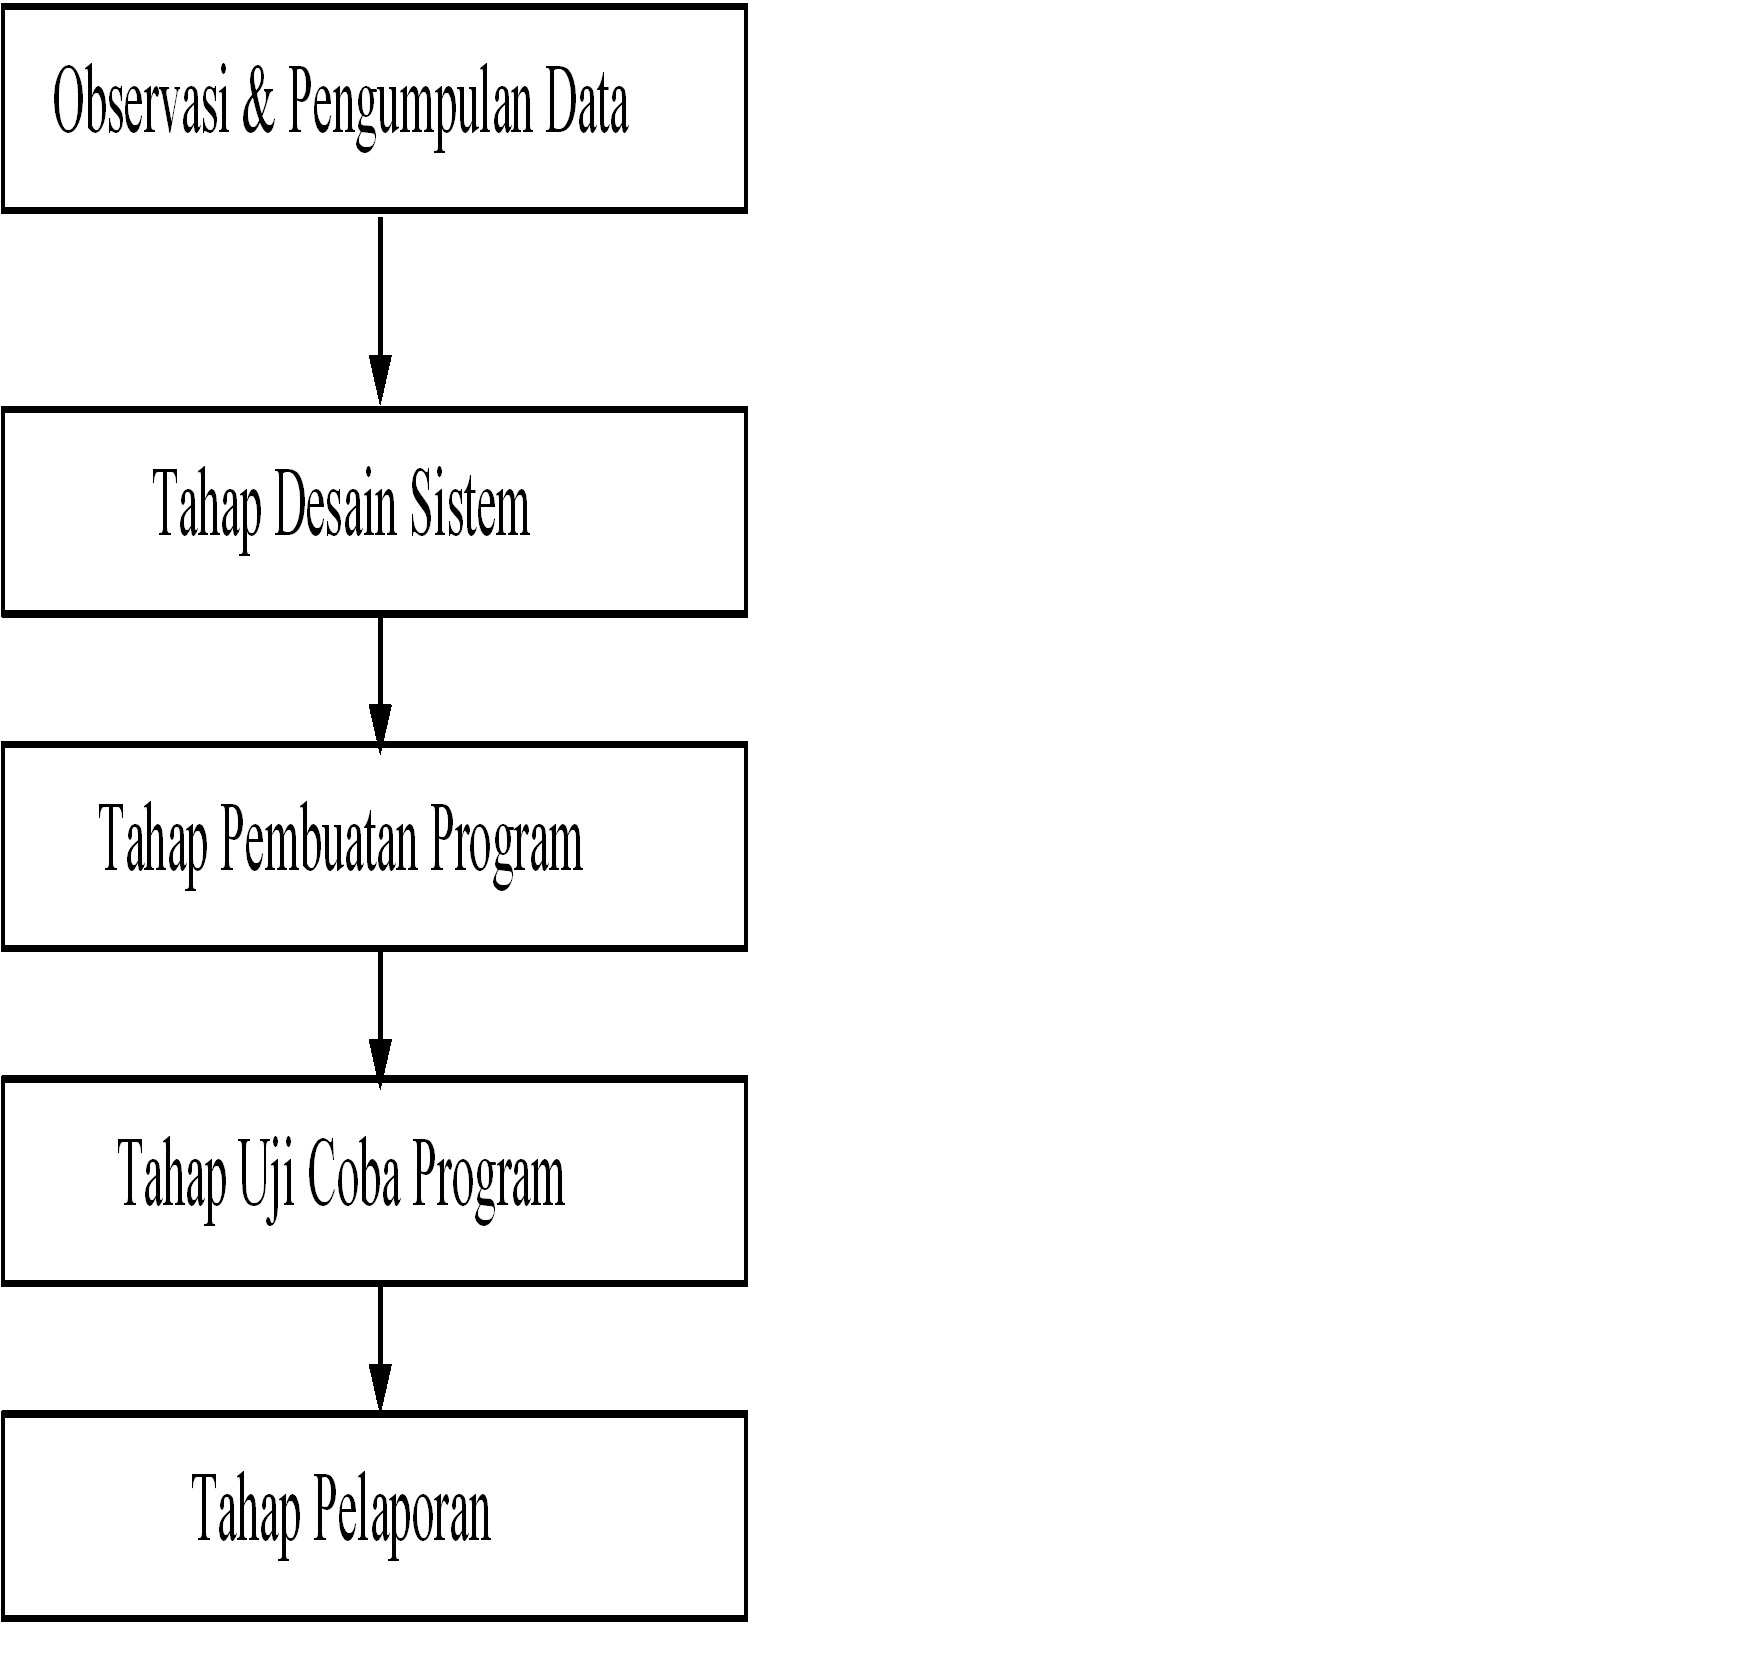
\includegraphics[width=0.7\textwidth]{gambar/1}  
 \caption{Tampilan Flowchart Pembuatan Proposal}
\end{figure}
\newpage
\section{Flowchart Pengembangan Sistem}
\begin{figure}[h]
\centering 
 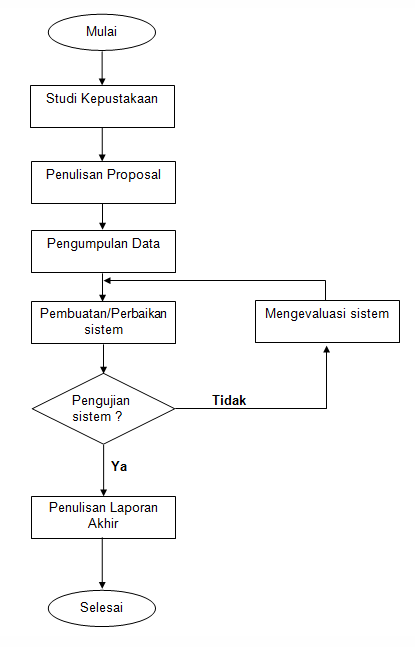
\includegraphics[width=0.5\textwidth]{gambar/2}  
 \caption{Tampilan Flowchart Pengembangan Sistem}
\end{figure}
\newpage
\section{Jadwal Kegiatan}
Penelitian direncanakan akan dilaksanakan selama empat bulan. Rincian rencana jadwal penelitian dicantumkan dalam tabel berikut.

\begin{center}
Tabel 3.1. Jadwal Penelitian.
\end{center}
\vspace{-0.5cm}
\begin{figure}[ht!]
  \centering
    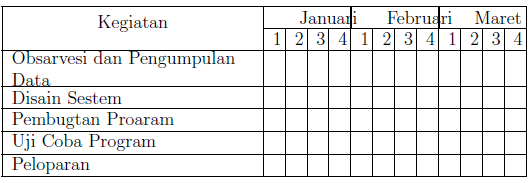
\includegraphics[width=13cm]{gambar/3}
\end{figure}

%-----------------------------------------------------------------
%Disini akhir masukan Bab
%-----------------------------------------------------------------

%-----------------------------------------------------------------
%Disini awal masukan untuk Daftar Pustaka
%-----------------------------------------------------------------
%%\nocite{Abel2010,Guerbas201350}
%%\bibliography{research-plan}
%%\bibliographystyle{plainnat}
\begin{thebibliography}{9}

\bibitem[satu(2013)]{satu01}
Budi Raharjo, Imam Heryanto, Arif Haryono, Mudah Belajar php. Bandung : Informatika
\bibitem[dua(2013)]{dua02}
Supardi, Yanuar, Ir. 2007. Pemrograman Database dengan Java dan MySQL, Jakarta : PT.Gramedia.
\bibitem[tiga(2013)]{tiga03}
Hariyanto, Bambang, Ir, MT. 2003, Esensi-esensi Bahasa Pemrograman mysql. Bandung : Informatika
\bibitem[empat(2013)]{empat04}
Dokumen online, www.wikipedia.com/sistem-informasi-manajemen.html, Sistem Informasi Manajemen, diakses pada Januari 2014

\bibitem[lima(2013)]{lima05}
Dokumen online, www.sharingilmujava.com/sistem-manajemen-keseretariatan-oraganisasi.html, Sistem, diakses pada Desember 2014

\end{thebibliography}
\addcontentsline{toc}{chapter}{DAFTAR PUSTAKA}
%-----------------------------------------------------------------
%Disini akhir masukan Daftar Pustaka
%-----------------------------------------------------------------

\end{document}